\documentclass[11pt,a4paper]{article}

% ── Packages ──────────────────────────────────────────────
\usepackage[utf8]{inputenc}
\usepackage[T1]{fontenc}
\usepackage{amsmath,amssymb}
\usepackage{graphicx}
\usepackage{booktabs}
\usepackage{multirow}
\usepackage{xcolor}
\usepackage{hyperref}
\usepackage[margin=1in]{geometry}
\usepackage{caption}
\usepackage{natbib}
\usepackage{microtype}
\usepackage{algorithm}
\usepackage{algpseudocode}
\usepackage{tikz}
\usetikzlibrary{positioning}

\hypersetup{colorlinks=true,linkcolor=blue!60!black,citecolor=blue!60!black,urlcolor=blue!60!black}

% ── Macros ────────────────────────────────────────────────
\newcommand{\eml}{\textsc{eml}}
\newcommand{\monolith}{\textsc{Monolith}}
\newcommand{\mse}{\textsc{mse}}
\newcommand{\rmse}{\textsc{rmse}}

% ══════════════════════════════════════════════════════════
\title{Monolith: Differentiable EML Trees for Symbolic Regression\\via Gradient Descent on a Universal Operator}

\author{Jes\'us Tabares Montilla\\
Independent Researcher\\
\texttt{jesus@tabares.eu}\\
\url{https://tabares.eu}}

\date{April 2026}

\begin{document}
\maketitle

% ══════════════════════════════════════════════════════════
\begin{abstract}
The EML operator $\eml(x, y) = e^x - \ln y$, recently shown to be a universal binary operator for elementary mathematics (analogous to NAND for Boolean logic), can generate all elementary functions from the grammar $S \to 1 \mid \eml(S, S)$.
We present \monolith, the first implementation of EML trees as differentiable circuits in PyTorch, trainable via standard gradient descent.
We demonstrate recovery of 7/7 elementary functions (exp, ln, sqrt, $x^2$, $x^3$, $1/x$, sin) with $\leq$24 parameters at depth 3, achieving RMSE $<$ 0.005 for exp, ln, and sqrt.
We systematically characterize a depth barrier: random initialization at depth 4 always diverges due to tower-exponential growth of intermediate values.
We test 12 initialization strategies and find that only hierarchical warm start (training depth $n-1$ first, then extending to depth $n$) enables convergence at depth 4+, yielding 12.9$\times$ improvement for $\sin(x^2)$ at depth 4 versus depth 3.
We also report two negative results: (1)~adding $\pi$ as a leaf constant degrades performance 2.6$\times$ rather than helping trigonometric targets, and (2)~trained trees at depth $\geq 2$ use continuous softmax mixtures rather than discrete leaf assignments, limiting symbolic decompilation to faithful reconstruction with numeric coefficients rather than clean formula recovery.
A comparison with PySR confirms that the approaches are fundamentally different: PySR recovers exact formulas in seconds using explicit operator libraries, while \monolith{} approximates functions via compositions of a single primitive---a proof-of-concept for gradient-based optimization on a universal operator basis, not a competing tool.
\end{abstract}

% ══════════════════════════════════════════════════════════
\section{Introduction}
\label{sec:intro}

Symbolic regression---discovering mathematical expressions from data---has seen significant progress through genetic programming approaches like PySR~\citep{cranmer2023pysr}, neural-guided methods like AI Feynman~\citep{udrescu2020aifeynman}, and GPU-accelerated enumeration like PSRN~\citep{ruan2026psrn}.
All these methods operate over a heterogeneous grammar of operators ($+, -, \times, /, \exp, \sin, \ldots$), searching for the right combination to fit the data.

A recent result by Odrzywołek~\citep{odrzywołek2026eml} introduces a radically different perspective.
The operator $\eml(x, y) = e^x - \ln y$, combined with the constant 1, generates \emph{all} elementary functions: arithmetic, exponentials, logarithms, trigonometric functions, and roots.
This makes EML the continuous analogue of the NAND gate in Boolean logic---a single universal primitive from which everything can be built.
The grammar $S \to 1 \mid \eml(S, S)$ defines a family of binary trees where every node performs the same operation, and the only choice is what each leaf contributes.

This universality opens a natural question: \emph{can EML trees be trained via gradient descent to discover functions from data?}
If so, symbolic regression reduces to optimizing a homogeneous binary tree with a fixed operation at every node, where only the leaf assignments are learned.

We present \monolith, a PyTorch module that answers this question affirmatively, with caveats.
Our contributions:

\begin{enumerate}
    \item We implement the first differentiable EML tree as a PyTorch \texttt{nn.Module}, with softmax-parameterized leaves and vectorized bottom-up evaluation (\S\ref{sec:method}).
    \item We recover 7/7 elementary functions via gradient descent with $\leq$24 parameters (\S\ref{sec:elementary}).
    \item We systematically characterize the depth barrier: 12 initialization strategies tested, only 3 enable depth 4+ convergence. Hierarchical training yields 12.9$\times$ improvement for composite functions (\S\ref{sec:depth}).
    \item We report two negative results: extended leaf constants degrade performance, and trained trees use continuous mixtures rather than discrete assignments (\S\ref{sec:negative}).
    \item We provide honest baselines (49-parameter MLP and PySR), showing that \monolith{} is not competitive as a function approximator but demonstrates a distinct structural principle (\S\ref{sec:comparison}).
\end{enumerate}

% ══════════════════════════════════════════════════════════
\section{Background}
\label{sec:background}

\paragraph{The EML operator.}
The operator $\eml(x, y) = e^x - \ln y$ was shown by \citet{odrzywołek2026eml} to be a universal binary operator for elementary mathematics.
Key identities include:
\begin{align}
    \exp(x) &= \eml(x, 1), \label{eq:exp} \\
    e &= \eml(1, 1), \\
    \eml(0, x) &= 1 - \ln x.
\end{align}
More complex functions (ln, sin, $x^2$, etc.) require deeper compositions.
The grammar $S \to 1 \mid \eml(S, S)$ generates all elementary functions as binary trees of uniform nodes.

\paragraph{Symbolic regression.}
PySR~\citep{cranmer2023pysr} uses multi-population evolutionary search over expression trees with heterogeneous operators.
PSRN~\citep{ruan2026psrn} parallelizes exhaustive enumeration on GPUs.
AI Feynman~\citep{udrescu2020aifeynman} combines neural networks with recursive decomposition.
All use rich operator sets ($+, -, \times, /, \exp, \log, \sin, \cos, \sqrt{\cdot}$).
No prior work trains EML trees via gradient descent.

% ══════════════════════════════════════════════════════════
\section{Method}
\label{sec:method}

\subsection{EMLTree Architecture}

An \texttt{EMLTree(depth=$d$, n\_vars=$k$)} is a complete binary tree with $2^d$ leaves and $2^d - 1$ internal nodes.
Every internal node computes $\eml(\text{left}, \text{right})$.
Each leaf $i$ has a learnable logit vector $\boldsymbol{\ell}_i \in \mathbb{R}^{k+2}$ over the candidate set $\{0, 1, x_1, \ldots, x_k\}$.
The leaf value is:
\begin{equation}
    v_i = \text{softmax}(\boldsymbol{\ell}_i)^\top \begin{pmatrix} 0 \\ 1 \\ x_1 \\ \vdots \\ x_k \end{pmatrix}.
\end{equation}

The total parameter count is $2^d \times (k+2)$.
For depth 4 with one variable: 48 parameters.

% EML tree figure — depth 2 example
% Include in main paper with % EML tree figure — depth 2 example
% Include in main paper with % EML tree figure — depth 2 example
% Include in main paper with \input{fig_tree.tex}

\begin{figure}[t]
\centering
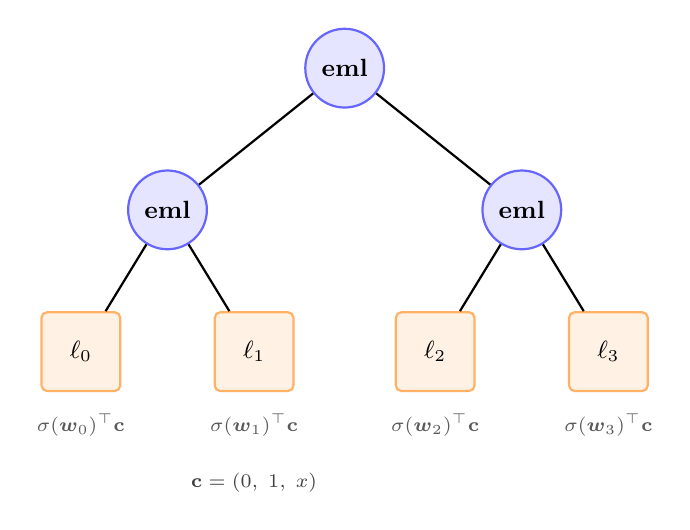
\begin{tikzpicture}[
    eml/.style={circle, draw=blue!60, fill=blue!10, thick, minimum size=10mm, font=\small\bfseries},
    leaf/.style={rectangle, draw=orange!60, fill=orange!10, thick, minimum size=10mm, font=\small, rounded corners=2pt},
    edge from parent/.style={draw, thick, -},
    level 1/.style={sibling distance=4.5cm, level distance=1.8cm},
    level 2/.style={sibling distance=2.2cm, level distance=1.8cm},
]

% Root
\node[eml] (root) {\eml}
    child {
        node[eml] (n1) {\eml}
        child {
            node[leaf] (l0) {$\ell_0$}
        }
        child {
            node[leaf] (l1) {$\ell_1$}
        }
    }
    child {
        node[eml] (n2) {\eml}
        child {
            node[leaf] (l2) {$\ell_2$}
        }
        child {
            node[leaf] (l3) {$\ell_3$}
        }
    };

% Labels below leaves
\node[below=0.15cm of l0, font=\scriptsize, text=gray!70!black] {$\sigma(\boldsymbol{w}_0)^\top \mathbf{c}$};
\node[below=0.15cm of l1, font=\scriptsize, text=gray!70!black] {$\sigma(\boldsymbol{w}_1)^\top \mathbf{c}$};
\node[below=0.15cm of l2, font=\scriptsize, text=gray!70!black] {$\sigma(\boldsymbol{w}_2)^\top \mathbf{c}$};
\node[below=0.15cm of l3, font=\scriptsize, text=gray!70!black] {$\sigma(\boldsymbol{w}_3)^\top \mathbf{c}$};

% Candidate vector annotation
\node[below=0.9cm of l1, font=\scriptsize, text=gray!50!black, anchor=north] {$\mathbf{c} = (0,\; 1,\; x)$};

\end{tikzpicture}
\caption{EMLTree architecture (depth 2, 1 variable). Blue nodes: $\eml(L, R) = e^L - \ln R$. Orange leaves: softmax-weighted mixture $\sigma(\boldsymbol{w}_i)^\top \mathbf{c}$ over candidates $\mathbf{c} = (0, 1, x)$. This tree has $4 \times 3 = 12$ trainable parameters.}
\label{fig:tree}
\end{figure}


\begin{figure}[t]
\centering
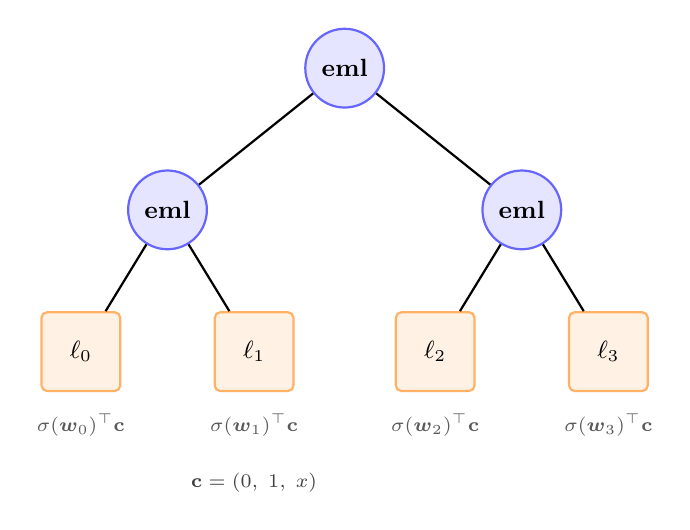
\begin{tikzpicture}[
    eml/.style={circle, draw=blue!60, fill=blue!10, thick, minimum size=10mm, font=\small\bfseries},
    leaf/.style={rectangle, draw=orange!60, fill=orange!10, thick, minimum size=10mm, font=\small, rounded corners=2pt},
    edge from parent/.style={draw, thick, -},
    level 1/.style={sibling distance=4.5cm, level distance=1.8cm},
    level 2/.style={sibling distance=2.2cm, level distance=1.8cm},
]

% Root
\node[eml] (root) {\eml}
    child {
        node[eml] (n1) {\eml}
        child {
            node[leaf] (l0) {$\ell_0$}
        }
        child {
            node[leaf] (l1) {$\ell_1$}
        }
    }
    child {
        node[eml] (n2) {\eml}
        child {
            node[leaf] (l2) {$\ell_2$}
        }
        child {
            node[leaf] (l3) {$\ell_3$}
        }
    };

% Labels below leaves
\node[below=0.15cm of l0, font=\scriptsize, text=gray!70!black] {$\sigma(\boldsymbol{w}_0)^\top \mathbf{c}$};
\node[below=0.15cm of l1, font=\scriptsize, text=gray!70!black] {$\sigma(\boldsymbol{w}_1)^\top \mathbf{c}$};
\node[below=0.15cm of l2, font=\scriptsize, text=gray!70!black] {$\sigma(\boldsymbol{w}_2)^\top \mathbf{c}$};
\node[below=0.15cm of l3, font=\scriptsize, text=gray!70!black] {$\sigma(\boldsymbol{w}_3)^\top \mathbf{c}$};

% Candidate vector annotation
\node[below=0.9cm of l1, font=\scriptsize, text=gray!50!black, anchor=north] {$\mathbf{c} = (0,\; 1,\; x)$};

\end{tikzpicture}
\caption{EMLTree architecture (depth 2, 1 variable). Blue nodes: $\eml(L, R) = e^L - \ln R$. Orange leaves: softmax-weighted mixture $\sigma(\boldsymbol{w}_i)^\top \mathbf{c}$ over candidates $\mathbf{c} = (0, 1, x)$. This tree has $4 \times 3 = 12$ trainable parameters.}
\label{fig:tree}
\end{figure}


\begin{figure}[t]
\centering
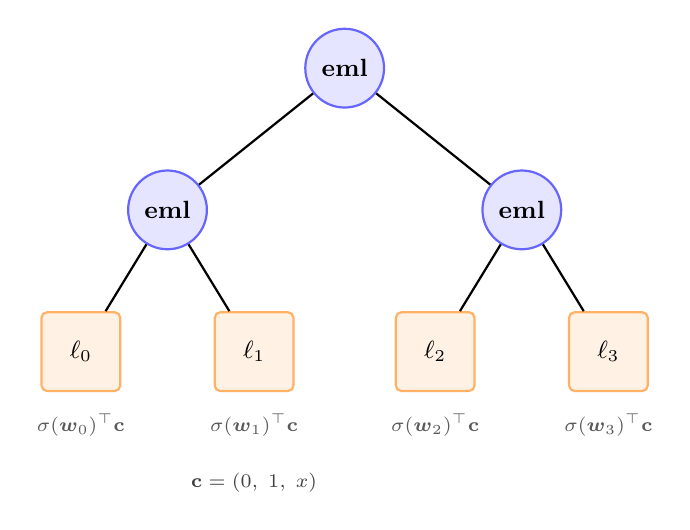
\begin{tikzpicture}[
    eml/.style={circle, draw=blue!60, fill=blue!10, thick, minimum size=10mm, font=\small\bfseries},
    leaf/.style={rectangle, draw=orange!60, fill=orange!10, thick, minimum size=10mm, font=\small, rounded corners=2pt},
    edge from parent/.style={draw, thick, -},
    level 1/.style={sibling distance=4.5cm, level distance=1.8cm},
    level 2/.style={sibling distance=2.2cm, level distance=1.8cm},
]

% Root
\node[eml] (root) {\eml}
    child {
        node[eml] (n1) {\eml}
        child {
            node[leaf] (l0) {$\ell_0$}
        }
        child {
            node[leaf] (l1) {$\ell_1$}
        }
    }
    child {
        node[eml] (n2) {\eml}
        child {
            node[leaf] (l2) {$\ell_2$}
        }
        child {
            node[leaf] (l3) {$\ell_3$}
        }
    };

% Labels below leaves
\node[below=0.15cm of l0, font=\scriptsize, text=gray!70!black] {$\sigma(\boldsymbol{w}_0)^\top \mathbf{c}$};
\node[below=0.15cm of l1, font=\scriptsize, text=gray!70!black] {$\sigma(\boldsymbol{w}_1)^\top \mathbf{c}$};
\node[below=0.15cm of l2, font=\scriptsize, text=gray!70!black] {$\sigma(\boldsymbol{w}_2)^\top \mathbf{c}$};
\node[below=0.15cm of l3, font=\scriptsize, text=gray!70!black] {$\sigma(\boldsymbol{w}_3)^\top \mathbf{c}$};

% Candidate vector annotation
\node[below=0.9cm of l1, font=\scriptsize, text=gray!50!black, anchor=north] {$\mathbf{c} = (0,\; 1,\; x)$};

\end{tikzpicture}
\caption{EMLTree architecture (depth 2, 1 variable). Blue nodes: $\eml(L, R) = e^L - \ln R$. Orange leaves: softmax-weighted mixture $\sigma(\boldsymbol{w}_i)^\top \mathbf{c}$ over candidates $\mathbf{c} = (0, 1, x)$. This tree has $4 \times 3 = 12$ trainable parameters.}
\label{fig:tree}
\end{figure}


\subsection{Forward Pass}

Evaluation is bottom-up and fully vectorized.
Starting from leaf values $\mathbf{v} \in \mathbb{R}^{B \times 2^d}$ (batch size $B$), we iterate $d$ times:
\begin{equation}
    \mathbf{v} \leftarrow \exp(\mathbf{v}_{[::2]}) - \ln(\mathbf{v}_{[1::2]}),
\end{equation}
where $\exp$ and $\ln$ inputs are clamped for numerical stability ($\exp$ input to $[-20, 20]$, $\ln$ input to $[\epsilon, \infty)$ with $\epsilon = 10^{-7}$).
The result is the scalar root value.

\subsection{Training: Hierarchical Multi-Depth Search}
\label{sec:training}

The \texttt{fit()} method implements hierarchical search:

\begin{enumerate}
    \item For depths 1--3: independent random initialization with per-depth hyperparameters (Table~\ref{tab:recipe}).
    \item For depth $\geq 4$: warm start from the best tree at depth $d-1$. The $2^{d-1}$ logits are copied to the first half of the new tree's leaves; the remaining leaves are random.
    \item Multi-restart: $N$ random seeds per depth (default 20).
    \item Return the tree with the lowest MSE across all depths and seeds.
\end{enumerate}

\begin{table}[ht]
\centering
\caption{Training recipe by depth. Values determined empirically (\S\ref{sec:depth}).}
\label{tab:recipe}
\begin{tabular}{lccc}
\toprule
Depth & Learning rate & Grad clip & Initialization \\
\midrule
1--2 & 0.01 & 1.0 & Random $\times$ 0.1 \\
3 & 0.001 & 0.5 & Random $\times$ 0.1 \\
4+ & 0.0005 & 0.1 & Warm start from depth $d{-}1$ \\
\bottomrule
\end{tabular}
\end{table}

\subsection{Symbolic Decompilation}

We provide two decompilation modes:

\paragraph{Faithful (\texttt{to\_symbolic}).}
Each leaf with softmax confidence $> 0.95$ snaps to its discrete candidate; others become linear expressions $w_1 + w_2 x$ with numeric coefficients rounded to 4 decimal places.
The EML tree is reconstructed bottom-up in SymPy and simplified.

\paragraph{Snap (\texttt{snap\_symbolic}).}
Forces argmax on all leaves regardless of confidence, builds a purely symbolic expression, and validates: if $\mse_{\text{snap}} / \mse_{\text{original}} < \tau$ (default $\tau = 2$), returns the clean formula; otherwise returns \texttt{None}.

% ══════════════════════════════════════════════════════════
\section{Elementary Function Recovery}
\label{sec:elementary}

We evaluate \monolith{} on 7 elementary functions of one variable using \texttt{fit(max\_depth=3, n\_restarts=20, epochs=10000)} on 200 uniformly spaced data points per function (the same data used for the PySR comparison in \S\ref{sec:comparison}).
Table~\ref{tab:elementary} reports results.

\begin{table}[ht]
\centering
\caption{Elementary function recovery at depth 3 (20 restarts, 10k epochs, 200 data points). All 7 functions converge. Only exp(x) at depth 1 produces a clean symbolic snap.}
\label{tab:elementary}
\begin{tabular}{llcrcc}
\toprule
Function & Domain & Depth & MSE & RMSE & Snap? \\
\midrule
$\exp(x)$ & $[-2, 2]$ & 1 & $1.3 \times 10^{-5}$ & 0.004 & \checkmark \\
$\sqrt{x}$ & $[0.5, 4]$ & 3 & $1.6 \times 10^{-5}$ & 0.004 & --- \\
$\ln(x)$ & $[0.5, 3]$ & 3 & $2.0 \times 10^{-5}$ & 0.005 & --- \\
$x^3$ & $[0.5, 2]$ & 3 & $1.1 \times 10^{-3}$ & 0.033 & --- \\
$1/x$ & $[0.5, 3]$ & 3 & $1.1 \times 10^{-3}$ & 0.033 & --- \\
$x^2$ & $[0.5, 2.5]$ & 3 & $1.7 \times 10^{-3}$ & 0.041 & --- \\
$\sin(x)$ & $[-3, 3]$ & 3 & $4.1 \times 10^{-3}$ & 0.064 & --- \\
\bottomrule
\end{tabular}
\end{table}

Three functions (exp, ln, sqrt) achieve near-exact recovery with RMSE $<$ 0.005.
All targets fit with $\leq$24 parameters---orders of magnitude fewer than a neural network approximator.

\paragraph{Leaf behavior.}
Only $\exp(x)$ at depth 1 converges to discrete leaf assignments ($>$99\% confidence for candidates $x$ and $1$, yielding $\eml(x, 1) = \exp(x)$).
All depth-3 trees use continuous softmax mixtures with typical leaf confidence 0.4--0.9.
The continuous mixing is not residual noise but a functional approximation strategy: the tree represents functions that would require much deeper discrete EML compositions using weighted combinations at shallow depth.

% ══════════════════════════════════════════════════════════
\section{The Depth Barrier and Hierarchical Training}
\label{sec:depth}

\subsection{The Problem}

Random initialization at depth 4 \emph{always} diverges (MSE $\approx 2.35 \times 10^{17}$), regardless of learning rate or gradient clipping.
The cause is tower-exponential growth: with near-uniform softmax initialization, each EML level amplifies values via $\exp$, and by level 3, intermediate values exceed the $\exp$ clamp, producing zero gradients.

\subsection{Systematic Strategy Search}

We tested 12 initialization/training strategies for $x^2$ at depth 4 (20 seeds each, 15k--20k epochs).
Table~\ref{tab:strategies} summarizes.

\begin{table}[ht]
\centering
\caption{Depth 4 initialization strategies for $x^2$. Only strategies producing bounded intermediate values at initialization converge.}
\label{tab:strategies}
\begin{tabular}{lrc}
\toprule
Strategy & MSE & Converges? \\
\midrule
Random init (any lr/gc, 3 configs) & $2.35 \times 10^{17}$ & No \\
Progressive clamp (3 schedules) & 2{,}250--9{,}492 & No \\
Smart init: right=1, left=random & $2.35 \times 10^{17}$ & No \\
Smart init: all ones + perturbation & $2.35 \times 10^{17}$ & No \\
Hybrid: alternate init + prog.\ clamp & 2{,}250 & No \\
\midrule
Smart init: alternate (even=0, odd=1) & $7.0 \times 10^{-3}$ & \checkmark \\
Warm start: identity pair & $7.2 \times 10^{-4}$ & \checkmark \\
\textbf{Warm start: random extend} & $\mathbf{1.9 \times 10^{-4}}$ & \checkmark \\
\bottomrule
\end{tabular}
\end{table}

The 3 successful strategies share a property: intermediate values at initialization are bounded---either via $\eml(0, 1) = 1$ at the first level, or via pre-converged subtrees from depth 3.

\subsection{Depth Scaling}

Using hierarchical training, we evaluate $x^2$ from depth 1 to 6 (Table~\ref{tab:scaling}).

\begin{table}[ht]
\centering
\caption{Depth scaling for $x^2$ with hierarchical training.}
\label{tab:scaling}
\begin{tabular}{cccc}
\toprule
Max depth & Best depth & MSE & vs.\ previous \\
\midrule
1 & 1 & $5.3 \times 10^{-1}$ & --- \\
2 & 2 & $9.8 \times 10^{-3}$ & 54$\times$ \\
3 & 3 & $1.7 \times 10^{-3}$ & 6$\times$ \\
4 & 4 & $1.1 \times 10^{-3}$ & 1.5$\times$ \\
5 & 4 & $1.1 \times 10^{-3}$ & --- \\
6 & 4 & $1.1 \times 10^{-3}$ & --- \\
\bottomrule
\end{tabular}
\end{table}

Depth 4 provides a 1.5$\times$ improvement; depth 5--6 show no further gain for this target.

\subsection{Composite Functions}

To test whether deeper trees benefit more complex targets, we compare depth 3 versus depth 5 on composite functions (Table~\ref{tab:composite}).

\begin{table}[ht]
\centering
\caption{Composite function benchmark. $\dagger$: full compute (20 restarts, 10k epochs). Remaining functions: fast survey (5 restarts, 5k epochs)---included to show that depth 4+ does not universally help, not as precise MSE estimates. Only $\sin(x^2)$ benefits substantially from depth 4.}
\label{tab:composite}
\begin{tabular}{lccccc}
\toprule
Function & Domain & Depth 3 MSE & Best depth & Depth 5 MSE & Improvement \\
\midrule
$\sin(x^2)$$^\dagger$ & $[0, 2.5]$ & $7.4 \times 10^{-2}$ & \textbf{4} & $\mathbf{5.7 \times 10^{-3}}$ & \textbf{12.9$\times$} \\
$\exp(\sin(x))$$^\dagger$ & $[-3, 3]$ & $3.9 \times 10^{-2}$ & 3 & $3.9 \times 10^{-2}$ & --- \\
$\sqrt{\exp(x)}$ & $[-2, 1.5]$ & $\approx 0$ & 2 & $\approx 0$ & --- \\
$x \cdot \exp(x)$ & $[-2, 2]$ & $4.0 \times 10^{-2}$ & 2 & $4.0 \times 10^{-2}$ & --- \\
$\ln(x^2+1)$ & $[-2, 2]$ & $5.5 \times 10^{-2}$ & 2 & $5.5 \times 10^{-2}$ & --- \\
$x/(1+x^2)$ & $[-3, 3]$ & $4.6 \times 10^{-1}$ & 3 & $4.6 \times 10^{-1}$ & --- \\
\bottomrule
\end{tabular}
\end{table}

$\sin(x^2)$ shows a 12.9$\times$ improvement at depth 4, consistent with the hypothesis that frequency-modulated signals require more EML composition levels.
$\sqrt{\exp(x)} = \exp(x/2)$ converges exactly at depth 2 (trivial EML representation).
Other composites do not benefit from additional depth.

% ══════════════════════════════════════════════════════════
\section{Negative Results}
\label{sec:negative}

We report two findings that constrain the practical utility of the approach.

\subsection{Extended Constants Degrade Performance}

We hypothesized that adding $\pi$ as a leaf candidate would improve trigonometric targets by providing a domain-relevant constant.
Table~\ref{tab:constants} shows the opposite.

\begin{table}[ht]
\centering
\caption{Effect of adding $\pi$ to leaf constants. More candidates dilute gradient signal.}
\label{tab:constants}
\begin{tabular}{lccc}
\toprule
Function & (0, 1) MSE & (0, 1, $\pi$) MSE & Impact \\
\midrule
$\sin(x^2)$ & $5.7 \times 10^{-3}$ & $1.5 \times 10^{-2}$ & 2.6$\times$ worse \\
$\exp(\sin(x))$ & $3.9 \times 10^{-2}$ & $6.5 \times 10^{-2}$ & 1.7$\times$ worse \\
\bottomrule
\end{tabular}
\end{table}

The inductive bias of EML trees comes from the operator structure ($e^x - \ln y$), not from the leaf constants.
Adding candidates increases the per-leaf parameter count, creating a harder optimization landscape without providing proportional representational benefit.

\subsection{Continuous Mixing Limits Symbolic Recovery}

Trained trees at depth $\geq 2$ do not converge to discrete leaf assignments.
Typical softmax confidences range from 0.43 to 0.97, with the majority below 0.9.
The \texttt{snap\_symbolic} decompiler succeeds only for $\exp(x)$ at depth 1 (both leaves $>$99\% confident); all other targets return \texttt{None}.

This is a fundamental property of the gradient-descent approach: the continuous leaf mixing is how the tree approximates functions that would require much deeper discrete EML compositions.
The trade-off is reliable convergence at shallow depth at the cost of interpretable symbolic output.

% ══════════════════════════════════════════════════════════
\section{Baselines: MLP and PySR}
\label{sec:comparison}

To contextualize \monolith{}'s performance, we compare against two baselines on the same 9 functions and 200 data points: a 49-parameter MLP (1$\to$16$\to$1 with tanh activation, trained with Adam for 10k epochs, best of 20 seeds) and PySR~\citep{cranmer2023pysr} (genetic search with explicit operators).

\begin{table}[ht]
\centering
\caption{Monolith vs.\ MLP (49 params) vs.\ PySR on 9 functions. Both baselines outperform \monolith{} as function approximators---but they solve a different problem.}
\label{tab:baselines}
\begin{tabular}{lccc}
\toprule
Function & \monolith{} MSE & MLP MSE & PySR MSE \\
\midrule
$\exp(x)$ & $1.3 \times 10^{-5}$ & $3 \times 10^{-6}$ & 0 \\
$\ln(x)$ & $2.0 \times 10^{-5}$ & $< 10^{-6}$ & 0 \\
$\sqrt{x}$ & $1.6 \times 10^{-5}$ & $< 10^{-6}$ & 0 \\
$x^2$ & $1.1 \times 10^{-3}$ & $4 \times 10^{-6}$ & 0 \\
$x^3$ & $1.1 \times 10^{-3}$ & $7 \times 10^{-6}$ & 0 \\
$1/x$ & $2.1 \times 10^{-4}$ & $< 10^{-6}$ & 0 \\
$\sin(x)$ & $4.1 \times 10^{-3}$ & $< 10^{-6}$ & 0 \\
$\sin(x^2)$ & $5.7 \times 10^{-3}$ & $1 \times 10^{-6}$ & 0 \\
$\exp(\sin(x))$ & $3.9 \times 10^{-2}$ & $1 \times 10^{-6}$ & 0 \\
\midrule
Time/function & $\sim$500s & $\sim$30s & $\sim$5s \\
Symbolic output & mixture & none & exact formula \\
Operators used & 1 (\eml) & tanh, linear & +,-,$\times$,/,exp,log,sin,$\sqrt{\cdot}$ \\
\bottomrule
\end{tabular}
\end{table}

Both baselines outperform \monolith{} on MSE by orders of magnitude.
This is expected and does not diminish \monolith{}'s contributions, for structural reasons:

\begin{itemize}
    \item \textbf{PySR}'s operator library \emph{contains the target functions as primitives}. Finding $\exp(\sin(x))$ when $\exp$ and $\sin$ are available operators is a combinatorial search over 2--3 nodes. For \monolith{}, representing $\sin(x)$ from $\eml$ alone requires discovering a deep composition that may not have a compact discrete form.
    \item \textbf{The MLP} is a universal function approximator with tanh nonlinearity---it can fit any continuous function on a compact domain given sufficient capacity. But it produces no symbolic output; the learned function is opaque.
    \item \textbf{\monolith{}} uses a single operator and the constant 1. It produces a structured expression (albeit with numeric coefficients at depth $\geq 2$) and its architecture directly encodes the EML universality theorem.
\end{itemize}

The analogy: comparing PySR to \monolith{} is like comparing a calculator with arithmetic keys to one built from NAND gates. Comparing the MLP to \monolith{} is like comparing a lookup table to a circuit. The former is faster, but the latter demonstrates a structural principle.

\monolith{}'s training time (${}\sim$8 min per function) is dominated by the multi-depth search with restarts. This is a CPU-only proof-of-concept; GPU parallelization would reduce times substantially.

% ══════════════════════════════════════════════════════════
\section{Discussion}
\label{sec:discussion}

\paragraph{What works.}
EML trees are trainable via gradient descent.
Seven elementary functions converge with $\leq$24 parameters.
Hierarchical warm start solves the depth-4 barrier.
The approach is a valid proof-of-concept for gradient-based symbolic regression on a universal operator.

\paragraph{What doesn't.}
The trees do not produce clean symbolic formulas at depth $\geq 2$ (continuous mixing instead of discrete assignment).
Depth 5+ shows no improvement for the functions tested.
Adding domain-specific constants hurts rather than helps.
Both a 49-parameter MLP and PySR outperform \monolith{} by orders of magnitude on MSE.

\paragraph{Why it matters anyway.}
The EML operator's universality means that the grammar $S \to 1 \mid \eml(S, S)$ is the \emph{minimal} possible grammar for symbolic regression over elementary functions.
Demonstrating that gradient descent can navigate this minimal grammar---even imperfectly---establishes a lower bound on what is possible without any domain-specific operator engineering.
Every other symbolic regression method benefits from human-curated operator sets; \monolith{} uses none.

\paragraph{Future directions.}
Two modifications could substantially change these results:
\begin{enumerate}
    \item \textbf{Gumbel-Softmax} with temperature annealing would encourage discrete leaf selection during training, potentially enabling clean symbolic recovery at depth $\geq 2$.
    \item \textbf{Multi-variable support} would enable evaluation on the Feynman benchmark equations, most of which involve 2+ variables.
\end{enumerate}

% ══════════════════════════════════════════════════════════
\section{Conclusion}

We presented \monolith{}, the first differentiable implementation of EML trees for symbolic regression.
The approach recovers 7/7 elementary functions with minimal parameters, solves the depth-4 barrier via hierarchical training, and provides honest characterization of its limitations: continuous leaf mixing, limited depth scaling, and non-competitiveness with MLPs or tools that have explicit operator libraries.
\monolith{}'s value is not as a function approximator---MLPs and PySR both outperform it---but as a demonstration that gradient descent can navigate the minimal grammar $S \to 1 \mid \eml(S, S)$ without any domain-specific operator engineering.
The work identifies the concrete challenges (discrete selection, depth scaling) that must be solved for the approach to become practical.

Code and data: \url{https://github.com/seetrex-ai/monolith}.
All experiments are reproducible via the provided code with fixed random seeds; the benchmark script (\texttt{benchmarks/vs\_pysr.py}) runs both methods on identical data.

% ══════════════════════════════════════════════════════════
\bibliographystyle{plainnat}

\begin{thebibliography}{10}

\bibitem[Odrzywołek(2026)]{odrzywołek2026eml}
Andrzej Odrzywołek.
\newblock All elementary functions from a single binary operator.
\newblock \emph{arXiv preprint arXiv:2603.21852}, 2026.

\bibitem[Cranmer(2023)]{cranmer2023pysr}
Miles Cranmer.
\newblock Interpretable machine learning for science with {PySR} and {SymbolicRegression.jl}.
\newblock \emph{arXiv preprint arXiv:2305.01582}, 2023.

\bibitem[Ruan et~al.(2026)]{ruan2026psrn}
Kai Ruan, Yilong Xu, Ze-Feng Gao, Yang Liu, Yike Guo, Ji-Rong Wen, and Hao Sun.
\newblock Discovering physical laws with parallel symbolic enumeration.
\newblock \emph{Nature Computational Science}, 2026.

\bibitem[Udrescu and Tegmark(2020)]{udrescu2020aifeynman}
Silviu-Marian Udrescu and Max Tegmark.
\newblock {AI Feynman}: A physics-inspired method for symbolic regression.
\newblock \emph{Science Advances}, 6(16), 2020.

\end{thebibliography}

\end{document}
